\documentclass[a4paper,11pt]{article}
\usepackage{graphicx, amsfonts, amstext, amsmath, amssymb, amsthm, authblk}
\usepackage{amsthm}
\usepackage{verbatim,rotating,enumitem}
\usepackage{color,pst-text,amsmath, amssymb, amsthm, pst-node, verbatim, subfigure}
\usepackage{multicol}
\usepackage{textcomp}
\usepackage[stable]{footmisc}
\usepackage{lscape}

% \usepackage[framed,numbered,autolinebreaks,useliterate]{mcode}
% \newtheorem{algorithm}{Algorithm}
% ========================================
% Packages for flow chart. 
% \usepackage[latin1]{inputenc}
% \usepackage{tikz}
% \usetikzlibrary{shapes,arrows}
% \usepackage{verbatim}
% \usepackage[active,tightpage]{preview}
% \PreviewEnvironment{tikzpicture}
% \setlength\PreviewBorder{5pt}%
% =======================================
% \newcommand{\h}{\hspace{.8cm}}
%opening


\author{A.H. Sheikh}

% \email{hanangul12@yahoo.co.uk}
% \affiliation{Delft Institute of Applied Mathematics, Delft University of
% Technology, Netherlands}
 
% \institution{Delft University of Technology, Netherlands}
% \title{Meeting discussion}
\title{Instruction for ADEF1 Solver Software}
\vspace{20cm}
\date{}
% \date{\today}
\begin{document}
%
\maketitle
%
\section{Introduction}
ADEF1 solver software is divided into two parts. Multilvel implementation
requires matrices at all levels from finest to coarsest. The data files are
constructed in Matlab and subsequently are written into \texttt{.DAT} files.
Important part of ADEF1 solver sotware is part which implements multilevel
preconditioner. This is implemented in \texttt{PETSc}, which calls the 
\texttt{.DAT} files on run time. 
\paragraph{Structure}
Main directory  \texttt{Adef1\_Software} contains two sub-directorows;
\texttt{ConstructDatFiles} and \texttt{PetscSolver}.\\
The directory \texttt{ConstructDatFiles} constructs data files. 
\section{Constructing DATA files}
Add the directory \texttt{ConstructDatFiles} to Matlab path also 
AddPath of your PETSC \texttt{matlab-bin} directory in matlab session
or adapt path in program \texttt{MainMarmousi.m}. \\
\par
Run the program \texttt{MainMarmousi.m} It will ask for options in an input
dialogue box. Those options are as following; \\
\begin{table}[h]
\begin{tabular}{ll}
\textbf{Frequency} $f$ & Give values f = 1, 10, 20 or 40\\
\textbf{Meshsize} & In terms of grid points per wavelenth. Choose 10 or 20. \\
\textbf{Real shift} & Real shift in complex shifted Laplace preconditioenrr
CSLP,\\
& choose whatever you want to use as CSLP.\\
\textbf{Imag. shift}& Imaginary shift in complex shifted Laplace
preconditioenrr CSLP, \\
& choose  whatever you want to use as CSLP.  \\
\textbf{Damping}& Damping parameter in equation.\\
\end{tabular}
\end{table}
THat program  construct discrete matrices according to provided options.
An example is shown in Figure \ref{fig:fig1}.
%
\begin{figure}[h]
\centering
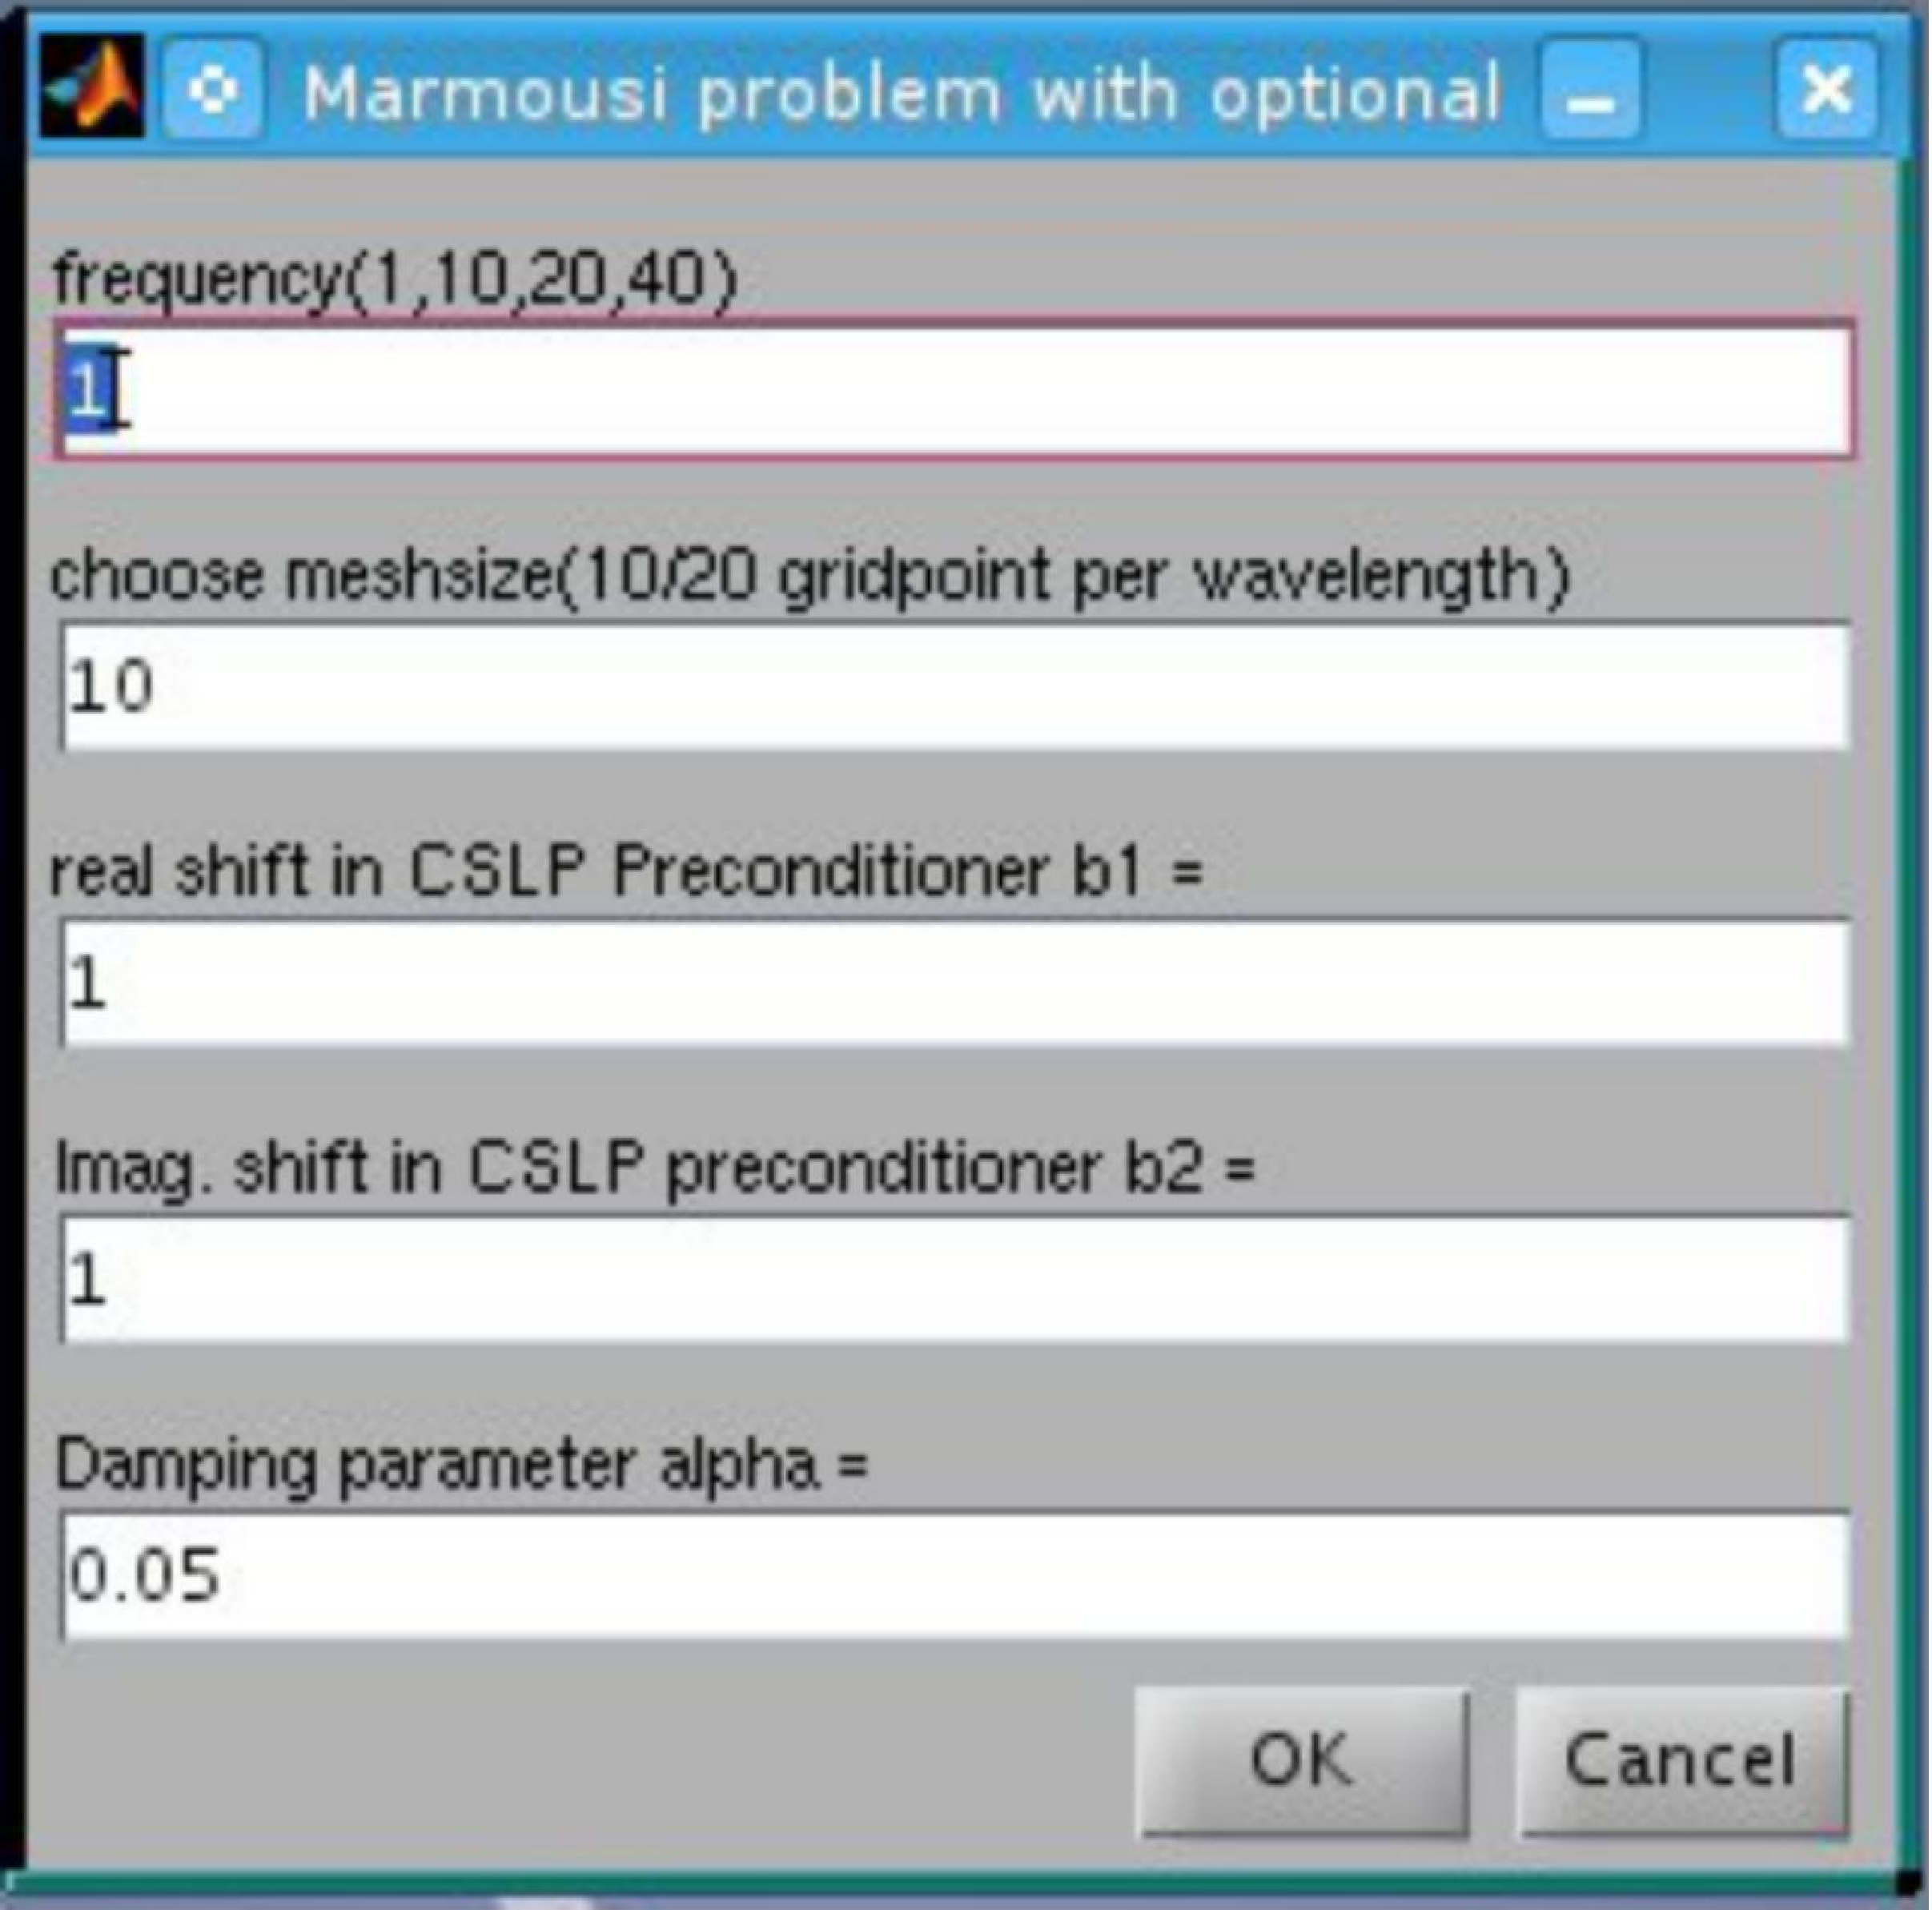
\includegraphics[width=7cm,height=5cm]{image1.pdf}
\caption{Menu to choose options while constructing \texttt{.DAT} files.}
\label{fig:fig1}
\end{figure}

\paragraph{Recommended:} First test run with defaults option in order to check
if it runs smoothly. Subsequently customize with options. \\
\par
Output file will be a .DAT file and will be saved in directory ../DAtaFiles/ 
with customized name \texttt{fN1gpWLN2aN3.dat} where f,gpWL,and
a are constant where N1, N2 and N3 will customized according to
options. For example f1gpWL10a0.05.dat, is data set with frequency $f=1$,
number of $gp/wl= 10$ and damping parameter $a = 0.05$. \\


\subsection{How to adapt}
PLEASE NOTE WHEN ADAPTING, \\
Reading \texttt{FILENAME.dat} file in Petsc is sensible of orders of
things(matrices and vectors) 
written in \texttt{.dat} file. If you wish to adapt, adapt it carefully. Take
care of the order, persist with same order while writing into .dat file and
reading same \texttt{.dat} file. \\
\par
The directory \texttt{PetscSolver} implements the ADEF1 solver.
\section{Solving part of software}
In the terminal, go to the target directory; Compile the program as follows\\

\texttt{> make GMGcycle.o; make MLadef.o; make MainSolver} \\

subsequntly execute the executable program and provide with data file with
``-f'' as follows: \\

\texttt{> ./MainSolver -f /your/path/to/datafile.dat}.\\ 
\par
This executuion accept all the possible runtime PETSc options. These all
options can be listen by executing program with ``-help''.
 



%
\end{document}
